\documentclass[a4paper,twoside]{article}
% My LaTeX preamble file - by Nathaniel Dene Hoffman
% Credit for much of this goes to Olivier Pieters (https://olivierpieters.be/tags/latex)
% and Gilles Castel (https://castel.dev)
% There are still some things to be done:
% 1. Update math commands using mathtools package (remove ddfrac command and just override)
% 2. Maybe abbreviate \imath somehow?
% 3. Possibly format for margin notes and set new margin sizes
% First, some encoding packages and useful formatting
%--------------------------------------------------------------------------------------------
\usepackage{import}
\usepackage{pdfpages}
\usepackage{transparent}
\usepackage[l2tabu,orthodox]{nag}   % force newer (and safer) LaTeX commands
\usepackage[utf8]{inputenc}         % set character set to support some UTF-8
                                    %   (unicode). Do NOT use this with
                                    %   XeTeX/LuaTeX!
\usepackage[T1]{fontenc}
\usepackage[english]{babel}         % multi-language support
\usepackage{sectsty}                % allow redefinition of section command formatting
\usepackage{tabularx}               % more table options
\usepackage{booktabs}
\usepackage{titling}                % allow redefinition of title formatting
\usepackage{imakeidx}               % create and index of words
\usepackage{xcolor}                 % more colour options
\usepackage{enumitem}               % more list formatting options
\usepackage{tocloft}                % redefine table of contents, new list like objects
\usepackage{subfiles}               % allow for multifile documents

% Next, let's deal with the whitespaces and margins
%--------------------------------------------------------------------------------------------
\usepackage[centering,margin=1in]{geometry}
\setlength{\parindent}{0cm}
\setlength{\parskip}{2ex plus 0.5ex minus 0.2ex} % whitespace between paragraphs

% Redefine \maketitle command with nicer formatting
%--------------------------------------------------------------------------------------------
\pretitle{
  \begin{flushright}         % align text to right
    \fontsize{40}{60}        % set font size and whitespace
    \usefont{OT1}{phv}{b}{n} % change the font to bold (b), normally shaped (n)
                             %   Helvetica (phv)
    \selectfont              % force LaTeX to search for metric in its mapping
                             %   corresponding to the above font size definition
}
\posttitle{
  \par                       % end paragraph
  \end{flushright}           % end right align
  \vskip 0.5em               % add vertical spacing of 0.5em
}
\preauthor{
  \begin{flushright}
    \large                   % font size
    \lineskip 0.5em          % inter line spacing
    \usefont{OT1}{phv}{m}{n}
}
\postauthor{
  \par
  \end{flushright}
}
\predate{
  \begin{flushright}
  \large
  \lineskip 0.5em
  \usefont{OT1}{phv}{m}{n}
}
\postdate{
  \par
  \end{flushright}
}

% Mathematics Packages
\usepackage[Gray,squaren,thinqspace,cdot]{SIunits}      % elegant units
\usepackage{amsmath}                                    % extensive math options
\usepackage{amsfonts}                                   % special math fonts
\usepackage{mathtools}                                  % useful formatting commands
\usepackage{amsthm}                                     % useful commands for building theorem environments
\usepackage{amssymb}                                    % lots of special math symbols
\usepackage{mathrsfs}                                   % fancy scripts letters
\usepackage{cancel}                                     % cancel lines in math
\usepackage{esint}                                      % fancy integral symbols
\usepackage{relsize}                                    % make math things bigger or smaller
%\usepackage{bm}                                         % bold math!
\usepackage{slashed}

\newcommand\ddfrac[2]{\frac{\displaystyle #1}{\displaystyle #2}}    % elegant fraction formatting
\allowdisplaybreaks[1]                                              % allow align environments to break on pages

% Ensure numbering is section-specific
%--------------------------------------------------------------------------------------------
\numberwithin{equation}{section}
\numberwithin{figure}{section}
\numberwithin{table}{section}

% Citations, references, and annotations
%--------------------------------------------------------------------------------------------
\usepackage[small,bf,hang]{caption}        % captions
\usepackage{subcaption}                    % adds subfigure & subcaption
\usepackage{sidecap}                       % adds side captions
\usepackage{hyperref}                      % add hyperlinks to references
\usepackage[noabbrev,nameinlink]{cleveref} % better references than default \ref
\usepackage{autonum}                       % only number referenced equations
\usepackage{url}                           % urls
\usepackage{cite}                          % well formed numeric citations
% format hyperlinks
\colorlet{linkcolour}{black}
\colorlet{urlcolour}{blue}
\hypersetup{colorlinks=true,
            linkcolor=linkcolour,
            citecolor=linkcolour,
            urlcolor=urlcolour}

% Plotting and Figures
%--------------------------------------------------------------------------------------------
\usepackage{tikz}          % advanced vector graphics
\usepackage{pgfplots}      % data plotting
\usepackage{pgfplotstable} % table plotting
\usepackage{placeins}      % display floats in correct sections
\usepackage{graphicx}      % include external graphics
\usepackage{longtable}     % process long tables

% use most recent version of pgfplots
\pgfplotsset{compat=newest}

% Misc.
%--------------------------------------------------------------------------------------------
\usepackage{todonotes}  % add to do notes
\usepackage{epstopdf}   % process eps-images
\usepackage{float}      % floats
\usepackage{stmaryrd}   % some more nice symbols
\usepackage{emptypage}  % suppress page numbers on empty pages
\usepackage{multicol}   % use this for creating pages with multiple columns
\usepackage{etoolbox}   % adds tags for environment endings
\usepackage{tcolorbox}  % pretty colored boxes!


% Custom Commands
%--------------------------------------------------------------------------------------------
\newcommand\hr{\noindent\rule[0.5ex]{\linewidth}{0.5pt}}                % horizontal line
\newcommand\N{\ensuremath{\mathbb{N}}}                                  % blackboard set characters
\newcommand\R{\ensuremath{\mathbb{R}}}
\newcommand\Z{\ensuremath{\mathbb{Z}}}
\newcommand\Q{\ensuremath{\mathbb{Q}}}
%\newcommand\C{\ensuremath{\mathbb{C}}}
\renewcommand{\arraystretch}{1.2}                                       % More space between table rows (could be 1.3)
\newcommand{\Cov}{\mathrm{Cov}}
\newcommand\D{\mathrm{D}}
\newcommand*{\dbar}{\ensuremath{\text{\dj}}}

\newcommand{\incfig}[2][1]{%
    \def\svgwidth{#1\columnwidth}
    \import{./figures/}{#2.pdf_tex}
}

% Custom Environments
%--------------------------------------------------------------------------------------------
\newcommand{\lecture}[3]{\hr\\{\centering{\large\textsc{Lecture #1: #3}}\\#2\\}\hr\markboth{Lecture #1: #3}{\rightmark}}   % command to title lectures
\usepackage{mdframed}
\theoremstyle{plain}
\newmdtheoremenv[nobreak]{theorem}{Theorem}[section]
\newtheorem{corollary}{Corollary}[theorem]
\newtheorem{lemma}[theorem]{Lemma}
\theoremstyle{definition}
\newtheorem*{ex}{Example}
\newmdtheoremenv[nobreak]{definition}{Definition}[section]
\theoremstyle{remark}
\newtheorem*{remark}{Remark}
\newtheorem*{claim}{Claim}
\AtEndEnvironment{ex}{\null\hfill$\diamond$}%
% Note: A proof environment is already provided in the amsthm package
\tcbuselibrary{breakable}
\newenvironment{note}[1]{\begin{tcolorbox}[
    arc=0mm,
    colback=white,
    colframe=white!60!black,
    title=#1,
    fonttitle=\sffamily,
    breakable
]}{\end{tcolorbox}}
\newenvironment{problem}{\begin{tcolorbox}[
    arc=0mm,
    breakable,
    colback=white,
    colframe=black
]}{\end{tcolorbox}}

% Header and Footer
%--------------------------------------------------------------------------------------------
% set header and footer
\usepackage{fancyhdr}                       % header and footer
\pagestyle{fancy}                           % use package
\fancyhf{}
\fancyhead[LE,RO]{\textsl{\rightmark}}      % E for even (left pages), O for odd (right pages)
\fancyfoot[LE,RO]{\thepage}
\fancyfoot[LO,RE]{\textsl{\leftmark}}
\setlength{\headheight}{15pt}


% Physics
%--------------------------------------------------------------------------------------------
\usepackage[arrowdel]{physics}      % all the usual useful physics commands
\usepackage{feyn}                   % for drawing Feynman diagrams
%\usepackage{bohr}                   % for drawing Bohr diagrams
%\usepackage{tikz-feynman}
\usepackage{elements}               % for quickly referencing information of various elements
\usepackage{tensor}                 % for writing tensors and chemical symbols

% Finishing touches
%--------------------------------------------------------------------------------------------
\author{Nathaniel D. Hoffman}

\title{33-761 Homework 4}
\date{\today}
\begin{document}
\maketitle

\section*{1. Solve Jackson Problem 2.10}%
\label{sec:solve_jackson_problem_2_10}
Note that, for parts (a) and (b) we are given that the separation $D$ between the two large plates is much much larger than the radius $a$ of the hemisphere. So we treat the plates as infinite and we may assume that the field at the far away plate is not affected by the hemispherical boss. This is a good approximation for the given problem. For part (c) we need multiple image charges to satisfy all the boundary conditions, but it is possible thanks to the symmetry of the problem.

\hr
A large parallel plate capacitor is made up of two plane conducting sheets with separation $D$, one of which has a small hemispherical boss of radius a on its inner surface ($D \gg a$). The conductor with the boss is kept at zero potential, and the other conductor is at a potential such that far from the boss the electric field between the plates is $E_0$.

\begin{itemize}
    \item[a)] Calculate the surface-charge densities at an arbitrary point on the plane and on the boss, and sketch their behavior as a function of distance (or angle).

        \begin{tcolorbox}[breakable]
    Because $D\gg a$, we will assume the region between the two plates has a uniform electric field $E_0$. To find the potential between the plates, we can imagine this as just the potential from a sphere in an electric field with certain boundary conditions for the plane. Jackson, in his infinite wisdom, shows how to calculate this in Section 2.5, and provides us with Equation 2.14:
    \begin{equation}
        \Phi = -E_0\left( r - \frac{a^3}{r^2} \right) \cos\theta
    \end{equation}

    To obtain an equation that works along the plane, we can factor out an $r$:
    \begin{equation}
        \Phi = -E_0 \left( 1-\frac{a^3}{r^3} \right) r\cos\theta 
    \end{equation}
    and note that if we let $r\cos\theta = z$, we will have a potential that vanishes both when $z=0$ and when $r=a$, the two boundary conditions we desire. Far from this conducting plane, this solution doesn't work, since we haven't factored in the second conductor, which won't have a constant field as is supposed in the problem (since $\Phi(D) = -E_0 D + E_0 \frac{a^3}{D^2}\cos\theta\neq -E_0 D$). However, it should work as a good approximation near the first plane, which is where we now want to calculate the surface-charge density.
    On the plane,
    \begin{equation}
        \sigma_{z=0} = -\epsilon_0\partial_z\Phi\eval_{z=0} = \epsilon_0E_0\partial_z\left(1-\frac{a^3}{r^3}z \right)\eval_{z=0} = \epsilon_0 E_0 \left( 1-\frac{a^3}{r^3} \right)
    \end{equation}
    On the boss,
    \begin{align}
        \sigma_{r=a} &= -\epsilon_0\partial_r\Phi\eval_{r=a} = \epsilon_0E_0\partial_r\left(r-0-\frac{a^3}{r^2}  \right)\cos\theta\eval_{r=a}\nonumber\\
        &= \epsilon_0E_0\left(1+2 \frac{a^3}{r^3} \right)\cos\theta\eval_{r=a} = 3\epsilon_0E_0\cos\theta
    \end{align}
    We can find the equivalent radial position along the boss by converting $\theta$ on the boss to the corresponding position on the plane. However, in our original system, $\theta$ was measured from the top of the boss. Here, $\sin\theta = \frac{r}{a}$ so $\cos\theta = \frac{\sqrt{a^2-r^2}}{a}$. We can check that this is correct since when $r=0$, we find this value to be $1=\cos\theta$, for $\theta = 0$ and $r=a$ gives us $0=\cos\theta$ for the points where the plane meets the boss. Therefore we can write these two solutions artificially using the same radial component (like we are looking at the charge distribution on the surface from the top down):
    \begin{equation}
        \sigma=
        \begin{cases}
            3\epsilon_0E_0 \frac{\sqrt{a^2-r^2}}{a} & r \le  a\\
            \epsilon_0E_0\left( 1-\frac{a^3}{r^3} \right) & r \ge a
        \end{cases}
    \end{equation}
    Below is a plot of the charge distribution as a function of radial position:
\end{tcolorbox}
\begin{figure}[h]
    \centering
    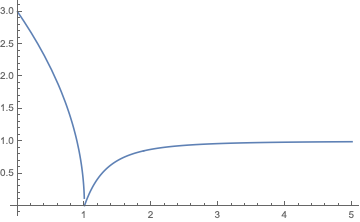
\includegraphics[width=0.8\textwidth]{hw_4_1a.png}
    \caption{Plot of Surface Charge Density as a Function of Radial Position ($a=E_0=\epsilon_0=1$ for convenience)}
    \label{fig:scd_plot}
\end{figure}

    \item[b)] Show that the total charge on the boss has the magnitude $3\pi\epsilon_0 E_0a^2$.

        \begin{tcolorbox}[breakable]
    For this, we just need to integrate the surface charge equation on the half-sphere:
    \begin{equation}
        3\epsilon_0 E_0\int_0^{2\pi}\int_0^{\frac{\pi}{2}}a^2\sin\theta\cos\theta d\theta = 3\epsilon_0 E_0 (2\pi) (\frac{a^2}{2}) = 3\pi\epsilon_0 E_0 a^2
    \end{equation}
    where $a^2$ comes from the integration factor $r^2\sin\theta$.
\end{tcolorbox}

    \item[c)] If, instead of the other conducting sheet at a different potential, a point charge $q$ is placed directly above the hemispherical boss at a distance $d$ from its center, show that the charge induced on the boss is
        \begin{equation}
            q' = -q \left[ 1- \frac{d^2-a^2}{d\sqrt{d^2+a^2}}\right] 
        \end{equation}

        \begin{tcolorbox}[breakable]
   We can use the method of images, but we must note that there are two surfaces which need to be taken into account. First, we must have an image charge for the plane, which we know must be at position $-d$ with charge $-q$. We must also have the image for the half-sphere at position $\frac{a^2}{d}$ with charge $q \frac{a}{d}$. Now to must also have an image for this charge on the other side of the flat plane, at position $-\frac{a^2}{d}$ with charge $-q \frac{a}{d}$. Our total potential is just the superposition of all of these potentials:
    \begin{equation}
        \begin{split}
            \Phi = \frac{1}{4\pi\epsilon_0}\left[&\frac{q}{\sqrt{x^2+y^2+(z-d)^2}} + \frac{-q}{\sqrt{x^2+y^2+(z+d)^2}}\right.\\
            &\left.+ \frac{q \frac{a}{d}}{\sqrt{x^2+y^2+(z-\frac{a^2}{d})^2} } + \frac{-q \frac{a}{d}}{\sqrt{x^2+y^2+(z+ \frac{a^2}{d})^2} } \right] 
        \end{split}
    \end{equation}

    We can then convert to spherical coordinates:

    \begin{equation}
        \begin{split}
            \Phi = \frac{1}{4\pi\epsilon_0}\left[& \frac{q}{\sqrt{r^2 + 2dr\cos\theta + d^2}} + \frac{-q}{\sqrt{r^2-2dr\cos\theta + d^2}}\right.\\
            &\left.+ \frac{q \frac{a}{d}}{\sqrt{r^2-2 \frac{a^2}{d}r\cos\theta + \left( \frac{a^2}{d} \right)^2}} + \frac{-q \frac{a}{d}}{\sqrt{r^2+2 \frac{a^2}{d}r\cos\theta + \left( \frac{a^2}{d}\right)^2}}\right]
        \end{split}
    \end{equation}
   
    Now we can calculate the surface charge of the boss
    \begin{equation}
        \sigma = -\epsilon_0\partial_r\Phi\eval_{r=a}
    \end{equation}
    and find the total induced charge by integrating this surface charge over the hemisphere:
    \begin{equation}
        q' = \int_0^{2\pi}d\phi\int_{\frac{\pi}{2}}^{\pi} -\epsilon_0\partial_r\Phi\eval_{r=a} a^2\sin\theta d\theta
    \end{equation}
    To be honest, I just put this all into Mathematica and got the correct answer, I don't think anyone is doing the derivative and integral by hand so there really isn't a point in showing the full derivation from here.
\end{tcolorbox}
\end{itemize}


\section*{2. Solve Jackson Problem 3.2}%
\label{sec:solve_jackson_problem_3_2}

There is symmetry around the $z$-axis so we expect that the solution can be expressed as an expansion in terms of $P_l(\cos\theta)$.

\hr

A spherical surface of radius $R$ has charge uniformly distributed over its surface with a density $ \frac{Q}{4\pi R^2}$, except for a spherical cap at the north pole, defined by the cone $\theta = \alpha$.

\begin{itemize}
    \item[a)] Show that the potential inside the spherical surface can be expressed as
        \begin{equation}
            \Phi = \frac{Q}{8\pi\epsilon_0}\sum_{l=0}^{\infty}\frac{1}{2l+1}[P_{l+1}(\cos\alpha)-P_{l-1}(\cos\alpha)] \frac{r^l}{R^{l+1}}P_l(\cos\theta)
        \end{equation}
        where, for $l=0$, $P_{l-1}(\cos\alpha) = -1$. What is the potential outside?

        \begin{tcolorbox}[breakable]
    We begin with an expansion of the potential for an azimuthally symmetric system. Inside the sphere, we expect the potential to behave well at $r=0$ and $r\to\infty$, so
    \begin{equation}
        \Phi = \begin{cases}
            \sum_{l=0}^{\infty} A_l \left( \frac{r}{R} \right)^{l}P_l(\cos\theta) & r<R\\
            \sum_{l=0}^{\infty} A_l \left( \frac{R}{r} \right)^{l+1}P_l(\cos\theta) & r>R 
        \end{cases}
    \end{equation}
    We must now find the proper coefficients for our system. For a charged surface, we expect $\sigma = \epsilon_0 (E_{r>R}-E_{r<R})\eval_{r=R} = -\epsilon_0(\partial_r\Phi_{r>R}-\Phi_{r<R})$:
    \begin{equation}
        \sigma = \sum_{l=0}^{\infty}\epsilon_0\left[\left( \frac{R}{r} \right)^{l+1} -  \left( \frac{r}{R} \right)^l \right]\eval_{r=R}A_l P_l(\cos\theta)
    \end{equation}
    or
    \begin{equation}
        \sigma = \sum_{l=0}^{\infty} \frac{2l+1}{R}A_l P_l(\cos\theta)
    \end{equation}

    By definition of the Legendre Polynomials, we know that
    \begin{equation}
        \int_{-1}^{1} P_l(\cos\theta)P_{l'}(\cos\theta)d(\cos\theta) = \left( \frac{2}{2l+1} \right)\delta_{l,l'}
    \end{equation}
    We can take the integral of each side of the previous equation with another Legendre polynomial:
    \begin{equation}
        \begin{split}
            \int_{-1}^{1}\sigma &P_l(\cos\theta)d(\cos\theta) =\\
            &\underbrace{\epsilon_0\sum_{l=0}^{\infty}\overbrace{\int_{-1}^{1}(\left( \frac{2l'+1}{R}A_{l'}P_{l'}(\cos\theta)\right)P_{l}(\cos\theta)d(\cos\theta)}^{\delta_{l,l'} \frac{2}{2l+1}\frac{2l'+1}{R}A_{l'}}}_{\frac{2\epsilon_0}{R}A_l}
        \end{split}
    \end{equation}
    So now we can solve for $A_l$ in terms of our known charge distribution:
    \begin{equation}
        A_l = \frac{R}{2\epsilon_0}\int_{-1}^{1}\sigma P_l(\cos\theta)d(\cos\theta)
    \end{equation}
    Our definitions for the charge distribution are based around the angle. Since we are only dealing with the range $\thepi\in[0,\pi]$, we know that $\cos\theta < \cos\alpha\iff\theta > \alpha$. Therefore,
    \begin{equation}
        \sigma = \begin{cases}
            \frac{Q}{4\pi R^2} & \cos\theta < \cos\alpha\\
            0 & \cos\theta > \cos\alpha
        \end{cases}
    \end{equation}
    This transforms the upper limit of the integral, since anything above $\cos\theta = \cos\alpha$ will not contribute to the integral, since the integrand will be zero:
    \begin{equation}
        A_l = \frac{R}{2\epsilon_0}\int_{-1}^{\cos\alpha} \frac{Q}{4\pi R^2}P_l(\cos\theta)d(\cos\theta)
    \end{equation}
    Moving the constants to the outside, we only have to evaluate the integral over the single Legendre polynomial. This can be done by the following general formula:
    \begin{equation}
        \int_{a}^{b} P_l(z)dz = \frac{P_{l+1}(z) - P_{l-1}(z)}{2l+1}\eval_{a}^{b}
    \end{equation}
    so
    \begin{equation}
        A_l = \frac{Q}{8\pi\epsilon_0 R}\frac{1}{2l+1}\left[ P_{l+1}(\cos\theta) - P_{l-1}(\cos\theta) \right]\eval_{-1}^{\cos\alpha}
    \end{equation}
    Rodrigues' Formula says that
    \begin{equation}
        P_n(x) = \frac{1}{2^n n!}(\partial_x)^n (x^2-1)^n
    \end{equation}
    so $P_l(-1) = (-1)^l$. Therefore,
    \begin{equation}
        A_l = \frac{Q}{8\pi\epsilon_0 R}\frac{1}{2l+1}\left[ P_{l+1}(\cos\alpha) - P_{l-1}(\cos\alpha) \right]
    \end{equation}
    were the condition that, for $l=0$, $P_{l-0}(\cos\alpha) = -1$ takes care of $P_0(-1) = 1$ (the other terms will be antisymmetric about $l$, $P_{l+1}(-1)-P_{l-1}(-1) = (-1)^{l+1}-(-1)^{l-1} = 0$ for $l\neq 0$).
    Substituting this back into the original equation for the potential inside the sphere gives the desired result.
\end{tcolorbox}

    \item[b)] Find the magnitude and the direction of the electric field at the origin.

        \begin{tcolorbox}[breakable]
            By symmetry, the electric field must point along the $z$-axis (or the axis from which $\alpha$ is measured). Because $\Phi\propto r^l$, $E\propto r^{l-1}$, so as $r\to 0$, only the $l=1$ term will be nonzero. Therefore,
            \begin{equation}
                E_{r=0,\theta=0} = \frac{Q}{8\pi\epsilon_0} \frac{1}{3}[P_2(\cos\alpha)-P_0(\cos\alpha)] \frac{1}{R^2}
            \end{equation}
            Evaluating the Legendre polynomials, we find
            \begin{equation}
                \vec{E} = \frac{Q}{16\pi\epsilon_0 R^2}(\cos^2\alpha - 1)\hat{z} = \frac{q\sin^2\alpha}{16\pi\epsilon_0 R^2}\hat{z}
            \end{equation}
        \end{tcolorbox}

    \item[c)] Discuss the limiting forms of the potential (part a) and electric field (part b) as the spherical cap becomes (1) very small, and (2) so large that the area with charge on it becomes a very small cap at the south pole.

        \begin{tcolorbox}[breakable]
            As $\alpha\to 0$,  $\cos\alpha\approx 1-\frac{1}{2}\alpha^2$ so
            $P_l(\cos\alpha)\approx P_l(1) -\frac{1}{2}a^2 P'_l(1)$ so $P_{l+1}(\cos\alpha)-P_{l-1}(\cos\alpha)\approx 2\delta_{l,0} - \frac{1}{2}\alpha^2[P'_{l+1}(1)-P'_{l-1}(1)] = 2\delta_{l,0} - \frac{1}{2}\alpha^2 (2l+1)P_l(1) = 2\delta_{l,0} - \frac{2l+1}{2}\alpha^2$.
            
            This makes the potential
            \begin{equation}
                \Phi\approx \frac{Q}{8\pi\epsilon_0}\left[\sum_{l=0}^{\infty}\left[2\delta_{l,0}-\frac{2l+1}{2}\alpha^2\right]\frac{1}{2l+1}\frac{r^l}{R^{l+1}}P_l(\cos\theta)\right] 
            \end{equation}
            or
            \begin{equation}
                \Phi\approx \frac{Q}{4\pi\epsilon_0}\frac{1}{R} - \frac{Q}{16\pi\epsilon_0}\sum_{l=0}^{\infty}\alpha^2 \frac{r^l}{R^{l+1}}P_l(\cos\theta)
            \end{equation}
            which is the potential inside a spherical shell with a slight correction that vanishes as $\alpha\to 0$. In the formulation of the electric field, this first term will vanish, leaving
            \begin{equation}
                E\approx\frac{Q\alpha^2}{16\pi\epsilon_0 R^2}
            \end{equation}
            As $\alpha\to\pi$, the system becomes a mostly uncharged sphere with a small cap of charge (on the south pole).
            We can do a similar expansion with some $\alpha' = \pi-\alpha$ and find the same results for $\alpha'$ that we found with $\alpha$ in the previous limiting case, although the direction will be reversed and the potential will just be the correction part without the term corresponding to the potential of a whole charged sphere. As we take $\alpha\to\pi$, we take $\alpha'\to 0$, so we find
            \begin{equation}
                \Phi\approx \frac{Q\alpha'^2}{16\pi\epsilon_0}\sum_{l=0}^{\infty} \frac{r^l}{R^{l+1}}P_l(\cos\theta)
            \end{equation}
            so
            \begin{equation}
                E\approx \frac{Q\alpha'^2}{16\pi\epsilon_0 R^2}
            \end{equation}
        \end{tcolorbox}
\end{itemize}

\section*{3. Solve Jackson Problem 3.6}%
\label{sec:solve_jackson_problem_3_6}

For part (a) due to symmetry around $z$-axis, express the result only in terms of $P_l(\cos\theta)$’s, not by means of $Y_{lm}(\theta,\phi)$ as Jackson originally asks. Thus for part (b) again, the limit should be taken using the expansion in part (a). Of course we can use the more general expansion but at this point it is not needed. [The more general expansion is useful if we have a dipole pointing in the $x$-direction and another charge, for example, placed at some point along the $z$-direction]. The answer to part (c) again is most naturally expressed by exploiting the symmetry around the $z$-axis.

\hr

Two point charges $q$ and $-q$ are located on the $z$ axis at $z=+a$ and $z=-a$, respectively.

\begin{itemize}
    \item[a)] Find the electrostatic potential as an expression in spherical harmonics and powers of $r$ for both $r>a$ and $r<a$.
   \begin{tcolorbox}
       The potential for two point charges in this configuration is
       \begin{equation}
           \Phi = \frac{q}{4\pi\epsilon_0}\left[\frac{1}{|\vec{x}-\vec{a}|} - \frac{1}{|\vec{x}+\vec{a}}\right] 
       \end{equation}

       We can expand each of these potentials as
       \begin{equation}
           \frac{1}{|\vec{x}-\vec{x}'|} = 4\pi\sum_{l,m} \frac{1}{2l+1}\frac{r^l_<}{r^{l+1}_>}Y^*_{lm}(\hat{x}')Y_{lm}(\hat{x})
       \end{equation}
       so
       \begin{equation}
           \Phi = \frac{q}{\epsilon_0}\sum_{l,m} \frac{1}{2l+1} \frac{r^l_<}{r^{l+1}_>}[Y^*_{lm}(0,\phi')-Y^*_{lm}(\pi,\phi')]Y_{lm}(\theta,\phi)
       \end{equation}
       From the azimuthal symmetry in the system, only the $m=0$ terms contribute. Additionally, $Y_{l 0}(0,\phi') = (-1)^lY_{l 0}(\pi,\phi') = \sqrt{\frac{2l+1}{4\pi}}$ by definition, so
       \begin{equation}
           \Phi = \frac{q}{4\pi\epsilon_0}\sum_{l=0}^{\infty}\frac{r^l_<}{r^{l+1}_>}[1-(-1)^l]\sqrt{\frac{2l+1}{4\pi}}\frac{1}{2l+1}Y_{l 0}(\theta,\phi) 
       \end{equation}
       Only the odd $l$ terms survive, and the $Y_{l 0}$ reduces to a Legendre polynomial:
       \begin{equation}
           \Phi = \frac{q}{2\pi\epsilon_0}\sum_{l=1,3,5, \ldots}\frac{r^l_<}{r^{l+1}_>}P_l(\cos\theta)
       \end{equation}
       or with slightly better notation
       \begin{equation}
           \Phi = \frac{q}{2\pi\epsilon_0}\sum_{l=0}\frac{r^{2l+1}_<}{r^{2l+2}_>}P_{2l+1}(\cos\theta)
       \end{equation}
   \end{tcolorbox} 
    \item[b)] Keeping the product $qa = \frac{p}{2}$ constant, take the limit of $a\to 0$ and find the potential for $r\neq 0$. This is by definition a dipole along the $z$ axis and its potential.
        \begin{tcolorbox}[breakable]
        Taking the limit, we know that the separation will be the smaller $r_<$, so
        \begin{equation}
            \Phi = \frac{q}{2\pi\epsilon_0}\sum_{l=0}\frac{a^{2l+1}}{r^{2l+2}}P_{2l+1}(\cos\theta)
        \end{equation}
        or
        \begin{equation}
            \Phi = \frac{qa}{2\pi\epsilon_0 r^2}\sum_{l=0}\left( \frac{a}{r} \right)^{2l}P_{2l+1}(\cos\theta) 
        \end{equation}
        So now if we take the limit $a\to 0$, setting $qa = \frac{p}{2}$, we find
        \begin{equation}
            \Phi = \frac{p}{4\pi\epsilon_0 r^2}P_1(\cos\theta) = \frac{p}{4\pi\epsilon_0}\frac{\cos\theta}{r^2}
        \end{equation}
    \end{tcolorbox}

    \item[c)] Suppose now that the dipole of part b is surrounded by a \textit{grounded} spherical shell of radius $b$ concentric with the origin. By linear superposition find the potential everywhere inside the shell.
        \begin{tcolorbox}[breakable]
            We can add a term to the potential to account for the shell:
            \begin{equation}
                \Phi = \frac{p}{4\pi\epsilon_0}\frac{\cos\theta}{r^2} + \sum_{l=0}^{\infty}A_l r^l P_l(\cos\theta) 
            \end{equation}
            The potential must be zero on the surface of the sphere (at $r=b$):
            \begin{equation}
                -\frac{p}{4\pi\epsilon_0}\frac{\cos\theta}{b^2} = \sum_{l=0}^{\infty} A_l b^l P_l(\cos\theta)
            \end{equation}
            By orthogonality of the Legendre polynomials, only the $l=1$ will survive (since $P_1(\cos\theta) = \cos\theta$ which is on the other side of the equation; I'm just matching powers of $\cos\theta$).
            \begin{equation}
                A_1 = -\frac{p}{4\pi\epsilon_0}\frac{1}{b^3}
            \end{equation}
            so
            \begin{equation}
                \Phi = \frac{p\cos\theta}{4\pi\epsilon_0}\left( \frac{1}{r^2} - \frac{r}{b^3} \right) 
            \end{equation}
        \end{tcolorbox}

\end{itemize}

\end{document}
